\documentclass[12pt,bibtotoc]{article}
\usepackage[table]{xcolor}
\usepackage[ngerman]{babel} % Für Silbentrennung
\usepackage[utf8]{inputenc} % Um Umlaute und Sonderzeichen nutzen zu können
\usepackage[a4paper,
lmargin={2cm},
rmargin={2cm},
tmargin={2cm},
bmargin={3cm}]{geometry} % Für das Layout
\usepackage{setspace} % Für den Zeilenabstand
\setstretch{1.25}
\usepackage{graphicx} % Um Bilder einzufügen
\usepackage{wrapfig} % Um Bilder im Fließtext einzubinden
\usepackage{csquotes} % Um Text in Anführungsstriche zu setzen
\usepackage{mathptmx} % Ähnlich zu Times New Roman
\usepackage{fancyhdr} % Um den Header einzufügen
\usepackage{pdfpages} % Um die Titelseite einbinden
\usepackage{hyperref} % Um Verlinkungen einfügen
\usepackage{acronym} % Um Akronyme zu definieren
\usepackage{textcomp} % Um spezielle Zeichen verwenden zu können (z.B. °, µ)
\usepackage{subcaption} % Um mehrere Bilder zusammen einzustellen und Links zu Abbildungen zu korrigieren
\usepackage{float}
\usepackage{placeins}
\usepackage{cleveref} %für Querverweise auf Kapitel: see section \cref{Kapitelname}

%Anpassung für itemize:
\usepackage{enumitem}
\setlist[itemize]{itemsep=0pt, topsep=0pt, leftmargin=1.5em}

\floatplacement{figure}{H}


\usepackage[backend=bibtex, citestyle=ieee]{biblatex} % Um Literatur einzufügen
\bibliography{Quellenverzeichnis}

\pagestyle{fancy}
\fancyhf{}
\setlength\headheight{59.76491pt}
\renewcommand{\headrulewidth}{0pt} % Um schwarze Linie zu entfernen
\chead{
\includegraphics[width=\textwidth]{Resources/header.png}} % Grafik einfügen
\cfoot{\thepage}

\newcounter{romanBeginningEnd} % Um Römische Seitenzahl zu speichern

% Sektionen refernezen anpassen
\addto\extrasngerman{%
	\renewcommand{\sectionautorefname}{siehe}%
	\let\subsectionautorefname\sectionautorefname%
	\let\subsubsectionautorefname\sectionautorefname%
}



\begin{document}
    \pagenumbering{gobble}
    \newpage




\definecolor{color_30879}{rgb}{0,0.12549,0.376471}
\vspace{20mm}
\noindent
{\fontsize{15.96}{1}\usefont{T1}{cmr}{m}{n}\selectfont\color{color_30879}Transferleistung Theorie/Praxis  }\\ 
{\fontsize{15.96}{1}\usefont{T1}{cmr}{m}{n}\selectfont\color{color_30879}Nr. 2} 

\vspace{15mm}



\begin{center}
\begin{tabular}{ |>{\columncolor{color_30879}}p{1.6in} | p{4.4in}| } 
 \hline
 \textcolor{white}{Martrikelnummer:} & 12657 \\[0.2in]
 \hline
 \textcolor{white}{Freigegebenes Thema:} & Wie kann Knk das optimale Hosting-Modell auswählen, das den spezifischen Anforderungen und Zielen des Kunden entspricht, um Kosten zu optimieren, Flexibilität sicherzustellen und gleichzeitig Sicherheits- und Compliance-Anforderungen gerecht zu werden? \\ [1in]
 \hline
 \textcolor{white}{Studiengang, Zenturie:} & Wirtschaftsinformatik, I22c \\ [0.2in]
 \hline
\end{tabular}
\end{center}

	%\includepdf[pages=-]{Resources/cover}
	
	\setcounter{page}{1} % Römische Seitenzahlen
	\pagenumbering{Roman}
	
	\tableofcontents %Inhaltsverzeichnis
	\newpage
	
	\setcounter{secnumdepth}{0} % Keine Numerierung von Überschriften
	\clearpage
	\phantomsection
	\addcontentsline{toc}{section}{\listfigurename} % Abbildungsverzeichnis im Inhaltsverzeichnis anzeigen
	\listoffigures
	\clearpage
	\phantomsection
	%\addcontentsline{toc}{section}{\listtablename} % Tabellenverzeichnis im Inhaltsverzeichnis anzeigen
	%\listoftables
	\newpage
	\section{Abkürzungsverzeichnis}
	% Abkürzungen
	\begin{acronym}[LängsteAbkürzung] % Für Formatierung längste Abkürzung eintragen
	\acro{ac:Label}[knk]{knk Business Software AG}
	\acro{ac:Label}[SaaS]{Software as a Service}
	\acro{ac:Label}[IaaS]{Infrastructure as a Service}
	\acro{ac:Label}[CRM]{Customer Relationship Management}
	\acro{ac:Label}[BC]{Business Central}
	\end{acronym}
	\newpage %Ich werde ganz sicherlich keine Abkürzungen einbauen um meine Transferlistung mit weniger Seiten zu bestücken. DAFUQ
	
	\setcounter{secnumdepth}{3} % Überschriften wieder numerieren
	
	\setcounter{romanBeginningEnd}{\the\value{page}} % Speichern der römischen Seitenzahl
	\setcounter{page}{1} % Mit Arabischen Seitenzahlen wieder bei 1 anfangen
	\pagenumbering{arabic}
	
	% ###############################################################
	% Tipps und Tricks:
	%\section{Begriffserklärung}
	%Beispieltext
	%\subsection{Was ist der Fachkräftemangel}
	%\newpage
	
	
	%\begin{figure}[h!]
		%\includegraphics[keepaspectratio,width=\textwidth,height=\textheight]{statistaEntwicklungFachkraefteindex.png} \renewcommand{\figurename}{Abb.}
		%\caption{\small Entwicklung des Fachkr{\"a}fteindex in Deutschland vom 1. Quartal 2015 bis zum 4. Quartal 2022; Hays über Statista, 2023}
	%\end{figure}
	
	%\cite{knk-info.2023}
	
	%\newpage
	
	% \begin{figure}[H] %Nutzung von Cloud Computing in Unternehmen in Deutschland in den Jahren 2011 bis 2022
	% 	\centering
	% 	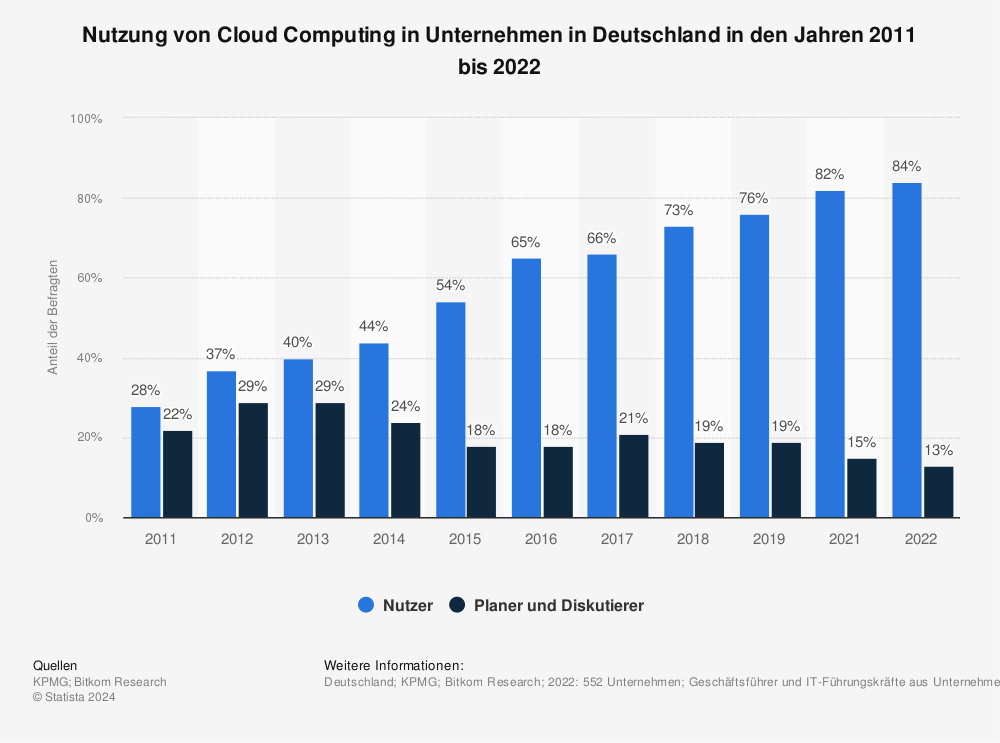
\includegraphics[keepaspectratio,width=\textwidth,height=\textheight]{"Content/Pictures/Nutzung von Cloud Computing in Unternehmen in Deutschland in den Jahren 2011 bis 2022.png"} 
	% 	\renewcommand{\figurename}{Abb.}
	% 	\caption{\small Nutzung von Cloud Computing in Unternehmen in Deutschland in den Jahren 2011 bis 2022}
	% \end{figure}
	
	%(\cite{Oelsnitz.2023}, Seite 4-5)
	
	%\begin{quote}
	%	,,Der aktuelle Wandel in Wirtschaft und Gesellschaft führt zu Umw{\"a}lzungen in einem bislang nicht gekannten Ausmaß. Strukturen, Prozesse, Aufgabenzuschnitte ver{\"a}ndern sich
	%	grundlegend – und dies in nahezu allen Branchen und Gesch{\"a}ftsbereichen.''\newline (\cite{Longmu.2021}, Seite 3)
	%\end{quote}

	%################################################################
	%Ab hier Inalt

	\section{Einleitung}
	%kleine Einleitung mit möglichen Methodenauflistung und einer groben Gliederungsbeschreibung?
	%möglicherweise eine Allgemeine Erklärung was Hosting-Modelle sind um den Leser bei den Anforderungsprofilen nicht zu überfordern?
	\subsection{Knk}
	Die Knk-Gruppe ist ein norddeutsches, international agierendes Unternehmen mit Hauptsitz in Kiel. Sie setzt sich aus den Unternehmen knk Business Software AG, der Business Unit muellerPrange, der knk Customer Engagement GmbH, der knk Cloud Services GmbH und Bradbury Phillips International zusammen. Hinzu kommen die knk Software LP (USA), knk Software Ltd. (UK) und knk France SAS (Frankreich)\cite{knk-info.2023}.
	\newline \newline
	Mit ihren Lösungen und Services innerhalb der Gruppe unterstützen sie Verlage und Medienunternehmen dabei, die Chancen der Digitalisierung und aktuelle Entwicklungen der Branche zu nutzen, Arbeitsabläufe zu optimieren und neue Zielgruppen zu erreichen. Im Fokus stehen hierbei neue Content-basierte Geschäftsmodelle, Business Intelligence und Künstliche Intelligenz für Verlage, CRM, Social Media Marketing sowie Marketing Automation\cite{knk-info.2023}.
	Das Produkt der knk Gruppe besteht aus dem Grundmodell von Business Central aus dem Hause Microsoft und wird in der ,,AL-Programming Language'' entwickelt und erweitert.
	\subsection{Hintergrund, Motivation und Zielsetzung der Transferleistung}
	Knk bietet schon lange Großprojekte für Medien- und Verlagshäuser in Form von KnkVerlag an. 
	Um nun auch kleinere Verlagshäuser anzusprechen, wurde knkMedia SaaS angekündigt und zur Verfügung gestellt \cite{knk-kuendigtSaaS-an.2023}.
	\newline
	knkMedia Saas soll schnelle aktualisierung innerhalb von Stunden ermöglichen und über die Microsoft-Cloud verfügbar sein.
	Die Vermarktung von knkMedia Saas als fertiges Produktpacket soll nun auch kleineren Verlagen mit 10 bis 20 Benutzern das ERP-System von Microsoft und die dazu passenden Knk-Erweiterungen attraktiver gestalten \cite{knk-kuendigtSaaS-an.2023}.
	\newline
	Die Motivation dieser Arbeit besteht darin, einen genaueren Überblick auf die verschiedenen Hostingmodelle zu bekommen und einen möglichst genauen Leitfaden zur Entscheidungsfindung aufzubauen.
	Der daraus entstehende Leeitfaden soll ermöglichen besser über Vor- und Nachteile informiert zu sein und bessere Entscheidungen aufgrund dieser zu treffen. 
	\newline
	Diese Transferleistung wird zwar auch allgemeine Fakten über Hosting-Modelle offenlegen, jedoch sich stark an Microsoft-Dienste orientieren um das von Microsoft entwickelte und von Knk erweiterte Business Central ERP-System 
	thematisch in den Vordergrund zu rücken. Zudem vertreibt Knk ihr Produkt nur in Verbindung mit Business Central.
	%möglicherweise erwähnen, dass es sich erstmal nur um BC dreht (check)
	%\subsection{Forschungsfrage} bietet aber vlt nicht genug


	\section{Anforderungsanalyse}
	\subsection{Erfassung der spezifischen Anforderungen von Knk und Kunden}
	%EI-Frage: Mir fällt keine ein. Thema streichen
	%vlt auch subsubsection
	\subsection{Technische und gesellschaftliche Anforderungen}

	\section{Hosting-Modelle im Überblick}
		\subsection{On-Premise}
		Bei einem On-Premise-Modell handelt es sich um eine lokal installierte Software, die auf jedem Computer eines Benutzers installiert werden muss, um die gewünschten Funktionalitäten zur Verfügung zu stellen.
		Meist sind auch die Daten, die eine Unternehmung für diese On-Premise-Sofware gebraucht auf lokalen oder Firmenweiten Datenbanken gespeichert \cite{AlHayek.2020}. 
		Bei Knk wird On-Premise Angeboten, wenn der Kunde bereit ist, eigene Server für die Software-Lösung bereit zu stellen /cite{Anhang}.
		\subsection{Cloud}
		%auf jedenfall noch mehr über die einzelnen Sachen schreiben
		%https://www.leanix.net/de/wiki/apm/saas-vs-cloud#What-is-cloud-based  Cloud ist überbegriff und SaaS ist eine unterkategorie. Das im SaaS-Kapitel hervorzeigen. 
		Cloud erntet immer mehr aufmerksamkeit und wird weitesgehend adaptiert. Als paradigmenwechsel in der IT betrachtet, wird es schon für vielfältige Anwedungsbereiche sowohl im geschäftlichen aber auch im privaten und behördlichen Bereich angewendet. \cite{Murugesan.2016}.
		\newline
		Die meisten privaten Nutzer, gebrauchen Cloud bereits um Fotos zu speichern oder für den eigenen Online-Kalendar sowie Online-Datenspeicherungen (z.B.: OneDrive)
		Klein- und Mittelgroße Unternehmen gebrauchen Cloud-Lösungen zum Beispiel für Cloud-basierte Anwedungen, Gehaltsabrechnungen, Kundenbeziehungsmanagement (CRM), Business Intelligence oder Datensammlung und Analyse.
		Großunternehmen nutzen Cloud-Dienste zum Beispiel für Geschäftsfunktionen wie Supply-Chain-Management, Datenspeicherung, Big-Data-Analysen, Geschäftsprozessmanagement, CRM oder Anwendungsentwicklung \cite{Murugesan.2016}.
		%nochmal sagen: Jo meist einfach Browser an und fertig der Lachs
		%\begin{singlespace} 
		\newline
			Es muss bei Cloud auf folgende Grundeigenschaften verwiesen werden \cite{Murugesan.2016}.
			\begin{itemize}
				\item Clouds stehen massive Ressourcen bei Bedarf zur Verfügung.
				\item Ressourcen können bedarfsgerecht skaliert werden.
				\item Sie bieten Ubiquität. Dies bedeutet, dass Daten unabhängig von Standort, Benutzer und Tageszeit zugänglich gemacht werden können.
				\item Es wird die gemeinsame Nutzung von Daten und unternehmensweite Datenanalyse sowie Zusammenarbeit gefördert.
				\item Clouds können sich bei Bedarf selbst rekonfigurieren um die Verfügbarkeit im Falle eines Ausfalls ihrer Datenverarbeitungsressourcen zu gewährleisten.
				\item Sie bieten eine vereinfachte Web-Browser-Oberfläche.
			\end{itemize}
		Diese Grundeigenschaften sind nur auf allgemeine Cloud-Lösungen beschränkt. \newline
		Bei Knk wird zwischen zwei Arten von Cloud unterschieden: Private-Cloud und SaaS-Cloud.
		%\end{singlespace}
		%herausfinden wie genau wir Cloud einsetzen, wer es dann hostet und wie es funktioniert und inwiefern es sich von SaaS abgrenzt.
		%auf jedenfall erwähnen seit wann Microsoft auch Cloud für BC anbietet
		\subsubsection{Private Cloud}
		Bei einer Private Cloud muss das betreibende Unternehmen selbst für den Betrieb, die Verwaltung und die Wartung der Software un dem dazugehörigen Clouddienst sorgen oder an einen Drittanbieter abtreten.
		Dabei muss die passende Software und die dazugehörigen Lizenzen eingekauft werden sowie Mitarbeiter für die Einrichtung der Software auf dem Cloud-Dienst an- oder abgestellt werden.
	Es wird meist ein Server bei einem Drittanbieter gemietet um die gewünschte Software darauf unterzubringen \cite{Anhang}. \newline
		Dies entspricht dem Geschäftsmodell von IaaS (Infrastructure as a Service) bei welchem Hardware wie Server, CPU, Speicher, Netzwerkausrüstung und Rechenzentrumseinrichtung, als Dienstleistung bereitgestellt wird.
		Anstatt diese Ressourcen also zu kaufen, erhalten die Kunden sie als vollständig ausgelagerte Dienstleistung für die Zeit in der sie sie benötigen \cite{Murugesan.2016}.
		\subsubsection{SaaS}
		Software as a Service, ist eine bestimmte Art der Nutzung von Cloud die auch Software-Clouds genannt werden. 
		Beim SaaS-Modell wird eine Anwendung von einem Cloud-Anbieter gehostet und als Service für die Nutzer bereitgestellt, in erster Linie über das Internet oder ein spezielles Netz.
		Es entfällt dadurch die Notwendigkeit, die Anwedung lokal auf dem Computer des Nutzers zu installieren und auszuführen und die Nutzer müssen sich nicht mehr um die Wartund und Aktualisierung der Hardware und Software kümmern.
		Den Nutzern wird dabei die genutzten Dienstleistungen in Rechnung gestellt. Somit werden die Kosten für die Nutzung eines Dienstes zu einer kontinuierlichen Ausgabe und nicht zu einer großen Anfangsinvestition zum Zeitpunkt des Kaufs \cite{Murugesan.2016}.
		%sind unterkategorie von Cloud-Lösungen. 
		
	\section{Detaillierter Vergleich der Hosting-Modelle}
			Durch die stationäre Bereitstellung der Umgebung und einer erforderten Installation des Produktes auf jedem Gerät ist bei On-Premise eine gewisse Flexibilität, nicht gegeben.
			Änderungen an der Software sorgen meist für einen gewissen Mehraufwand auf Seiten des Kunden und des Entwicklers. Dieser Mehraufwand ist bei Cloud nicht gegeben durch ein einfach nutzbares Browser-Interface und ein vergleichbar einfaches Roullout von Änderungen auf zugreifbare Server. 
			On-Premise beinhaltet daher Kostenkomponenten, die eine Eigenverantwortung für Faktoren wie Einrichtung des Servers vor Ort, Serversoftware, Arbeitsaufwand für die Systemadministatoren und andere Infrasrukturkosten beinhaltet, welche bei einem Cloud-Service in der Regel nicht anfallen \cite{Fisher.2018}.
			Nicht zu vergessen sind auch unerwartete Kosten aufgrund von Hardwareverschleiß oder anderen Begebenheiten, welche die Kosten in die Höhe treiben können, was durch die Eigenverantwortung durch On-Premise auf lange Sicht kaum zu vermeiden ist.
			\newline
			Sicherheit und Datenschutz ist ein weiterer Aspekt. Durch die lokale Speicherung der Daten bei On-Premise kann eine gewisse Macht über die eigenen Daten ausgeübt werden. 
			Bei Cloud-Lösungen wird diese Macht jedoch an den Host der Cloud-Server abgegeben der die Server zur Datenspeicherung besitzt. Dies kann im subjektiven Fall ein Problem darstellen. 
			\newline
			Die Skalierung der Ressourcen hebt Cloud maßgeblich von On-Prem ab. On-Prem bietet mit seinen lokalen Server eine meist feststehende beziehungsweise schwer zu erweiterbare Ressourcenstruktur. Braucht eine Unternehmung mit einem On-Prem-System eine 
			Ressourcenerweiterung, muss meist teure Hardware nachgekauft werden, was eine hohe einmalige Investition bedeutet.
			Bei Cloud wiederum, muss der Anbieter mehr Ressourcen frei geben, was zwar wieder eine höhere Bindung an den Cloud-Host bedeutet, jedoch auch eine vermeidung von Investitionen und je nach Anbieter lediglich eine Erhöhung der Gebühren zur Folge hat \cite{Murugesan.2016}.
			\newline
			\subsection{Faktoren für Knk und den Entwicklungsprozess}
			%Es muss auch erwähnt werden welche Aspekte dies für unsere Firma sind
			%%EI-Frage: Nachricht an Carsten: Hey Carsten. Ich habe eine Frage für meine TL: In welchen wesentlichen Aspekten unterscheidet sich der Rollout von Änderungen bei Kunden die On-Prem sind oder solchen die Cloud nutzen?
			Den Betrieb von On-Premise-Modellen geht meist ein tiefer technischer Zugriff einher. Beispielsweise ist der Zugriff auf die SQL-Datenbank direkt möglich. 
			Bei einem BC-Cloud-Modell ist dieser Zugriff nur über einen extra angerfertigten Admin-Bereich möglich der eingeschränkte Funktionalitäten im Gegensatz zu SQL bietet.
			Dieser technische Zugriff bietet ebenfalls eine bessere Möglichkeit, spezifische Anpassungen vorzunehmen wobei dies aber auch größere Verantwortung in Bezug auf Wartung und Verwaltung bedeutet \cite{Anhang}. \newline
			Private Cloud bietet im Gegensatz eine schnellere Installation von Apps und das Einspielen von AddOns. Dies reduziert sowohl Aufwand, als auch eine mögliche Beschleunigung der Implementierung von neuen Funktionen.
			Im Thema Performance bieten On-Premise-Server theoretisch eine höhre Rechenleistung. Jedoch sind diese Server in der Praxis oft stark ausgelastet, was die tatsächliche Leistung beeinträchtigen kann.
			Zudem muss bei der Arbeit mit verschiedenen Modellen, wie OnPrem und OnCloud, darauf geachtet werden, dass die gleichen Versionen von AddOns verwendet werden, um Konsistenz und Kompatibilität sicherzustellen \cite{Anhang}. \newline
			Schließlich erfordern Cloud-basierte Modelle oft den Einsatz neuer Werkzeuge und Methoden zur Administration. Administratoren müssen sich an diese neuen Werkzeuge gewöhnen, was zusätzlichen Schulungsaufwand mit sich bringen kann \cite{Anhang}.
			
			\newpage
			\subsection{Aktuelle Trends und Entwicklungen}
			%hierzu vlt auch nochmal bei PMS nachfragen, wie viele Projekte momentan zu Cloud wechseln. Vlt auch in einem Experteninterview oder so idk
			%Microsoft aktuelle Entwicklung vorheben gegenüber diesem Thema
			Die folgende Statisitk zeigt die Entwicklung der Cloud-Nutzung in deutschen Unternehmen zwischen 2011 und 2022.
			Dabei wird der Anteil der Unternehmen dargestellt, die Cloud-Dienste nutzen, sowie der Anteil der Unternehmen, die planen oder diskutieren, Cloud einzuführen. 
			\begin{figure}[H] %Nutzung von Cloud Computing in Unternehmen in Deutschland in den Jahren 2011 bis 2022
				\centering
				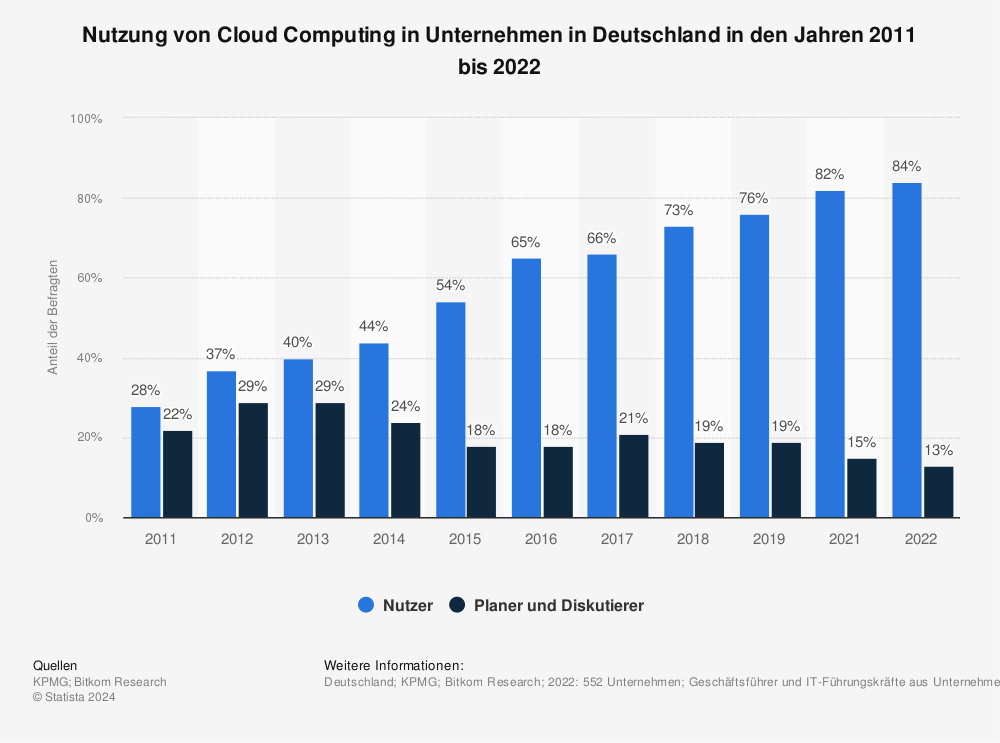
\includegraphics[keepaspectratio,width=\textwidth,height=\textheight]{"Content/Pictures/Nutzung von Cloud Computing in Unternehmen in Deutschland in den Jahren 2011 bis 2022.png"} 
				\renewcommand{\figurename}{Abb.}
				\caption{\small Nutzung von Cloud Computing in Unternehmen in Deutschland in den Jahren 2011 bis 2022}
			\end{figure}
			Die Statistik verdeutlicht, dass die Akzeptanz und Nutzung von Cloud in deutschen Unetrnehmen in den letzten Jahres bis 2022 erheblich gestiegen ist. 
			%EI-Frage: Was ist der zu beobachtende Trend von Kunden gegenüber der Entscheidung der Nutzung von Cloud oder On-Prem
			Beobachtet wird seitens Knk, dass ebenfalls immer mehr Kunden zu einer Private-Cloud oder SaaS-Lösung tendieren. Gerade Unternehmen, dessen Expertise nicht zentral zur IT gehört, bewegen sich in diese Richtung.
			Bei größeren Unternehmen wird jedoch auch auf On-Premise-Lösungen gesetzt, die einen gewissen höheren Spielraum für individuelle Lösungen bereit stellt und daher für Unternehmen dieser größe mit meist eigenen Anforderungen oder Geschäftsmodelle aufweisen, eine höhere Attraktivität bietet. \cite{Anhang}
			\newpage
			\section{Entwicklung von Entscheidungskriterien}
	Zunächst werden Kriterien aufgestellt und erläutert:
	\setlist{noitemsep}
	\begin{itemize}
		\item User-Anzahl %
		\begin{itemize}
			\item Die Anzahl der User innerhalb eines Unternehmens speilt eine große Rolle. Umso höher diese User-Anzahl, umso höher auch die einmaligen Anschaffungskosten bei On-Prem und/oder die Zahlungen für Cloud-Dienste.
		\end{itemize}
		\item Skalierbarkeit 
			\begin{itemize}
				\item In welchem Maße das eigene System skalierbar sein muss und wie viel Datenvolumen es bewältigen können soll.
			\end{itemize}
		\item Datenhoheit %
			\begin{itemize}
				\item Ist der Besitzer der Daten bereit, diese auch in die Hand von Drittanbietern zu legen.
			\end{itemize}
		\item Grad der individuellen Anpassungen %
			\begin{itemize}
				\item Je mehr Anpassungen erforderlich sind, desto eher wird ein On-Premise- oder Private-Cloud-Modell in Betracht gezogen.
			\end{itemize}
		\item Nutzung von Schnittstellen %
			\begin{itemize}
				\item Wenn viele oder spezielle Schnittstellen zwischen Programmen benötigt werden, bieten On-Premise oder Private-Cloud-Lösungen meist mehr Fleibilität beim Einbinden der benötigten Schnittstellen.
			\end{itemize}
		\item Bereits vorhandene Lizenzen %
			\begin{itemize}
				\item Welche Lizenzen schon bereits zur im Besitz des Kunden stehen, kann auch entscheiden welches Modell besser geeignet ist. 
			\end{itemize}
		\item Grad der Automatisierung %
			\begin{itemize}
				\item Hochgradig automatisierte Prozesse erfordern meist eine stabile und leistungsfähige Umgebung. 
			\end{itemize}
	\end{itemize}
	%!!!!!Vlt davon absehen hier schon eine Zuordnung zu den Modellen zu schreiben.
	%EI-Frage: Welche weitere Entscheidungskriterien tauchen bei Kunden häufig auf?
		\subsection{Gewichtung der Kriterien nach Relevanz}
		Aus den Vorangegangenen Informationen und dem Experteninterview mit Ansgar Pahl \cite{Anhang} geht folgende Soriterung der Kriterien hervor:
		\setlist{noitemsep}
		\begin{itemize}
			\item[1.] Grad der individuellen Anpassungen
			\item[2.] Gleichzeitig aktive User
			\item[3.] Skalierbarkeit (inkl. Datenmenge)
			\item[4.] Nutzung von Schnittstellen
			\item[5.] Bereits vorhandene Lizenzen
			\item[6.] Grad der Automatisierung
			\item[7.] Datenhoheit 
		\end{itemize}
		%EI-Frage: Was ist deiner Meinung nach das Relevanteste dieser Kriterien? 
		\subsection{Unterstützung für Unternehmen und Kunden bei der Auswahl}
		%auch erklären, dass Datenhoheit bei Microsoft keine Rolle spielt weil die Rechenzentrum in DE haben (braucht aber noch Quelle)

	\section{Praktische Beispiele aus der Industrie}
		%da brauche ich auf jedenfall ein Experteninterview. Vlt hat Arnold oder irgendein beratender Mensch zeit dafür?
		%EI-Frage: Welche Situationen fallen dir ein, in denen ein Kunde sich zwischen den beiden Modellen entscheiden musste und aus welchen Gründen, wurde das schlussendliche Modell ausgesucht? 
		Aus dem Experteninterview mit Ansgar Pahl \cite{Anhang}, gehen drei Fallbeispiele hervor die in den folgenden Unterkapiteln \ref{MVB}, \ref{Avoxa} und \ref{Sanoma} erläutert werden.
			\subsection{MVB}\label{MVB}
			Der ,,Marketing- und Verlagsservice des Buchhandels'' (MVB) ist ein Kunde von Knk mit Sitz in Frankfurt. Sie bieten Verlagsprodukte und Dienstleistungen an. Sie gehören zur Börsenvereinsgruppe \cite{MVB-Website.2024}.\newline 
			MVB begann zunächst damit bei Microsoft die Public-Business-Central-Cloud zu mieten und darüber das Produkt von Knk zu nutzen. Später jedoch entschied sich MVB dazu auf eine private Cloud in Azure umzusteigen, um den gewollten und erforderlichen Leistungszuwachs zu erzielen.
			\subsection{Avoxa}\label{Avoxa}
			Die ,,Avoxa-Mediengruppe deutscher Apotheker'' ist ein deutsches Medienunternehmen welches Zahlreiche Verlagsprodukte und Dienstleistungen im pharmazeutischen Bereich anbietet \cite{Avoxa-Website.2024}. \newline 
			Avoxa plante, IT-Personal und Hardware-Ressourcen im eigenen Unternehmen abzubauen. Der Verlag entschied sich aufgrunddessen dazu, in Zukunft eine Private-Cloud-Umgebung zu nutzen um die internen IT-Aufwände zu minimieren.
			\subsection{Sanoma}\label{Sanoma}
			Sanoma ist ein finnischer Medienkonzern. Sanomas bietet Angebote wie Zeitschriften, Zeitungen, Fernseh- und  Radiosender sowie Internetangebote im Bereich Bildung an \cite{Sanoma-Website.2024}. \newline
			Für Sanoma kam persönlich ausschließlich die BC-SaaS-Cloud in Frage. Um diese jedoch optimal zu nutzen, spielte die Integration einer Middleware, zur Kommunikation und Datenverwaltung zwischen verschiedenen Anwendung welche bei Sanoma genutzt werden, eine zentrale Rolle.
		%\subsection{Empfehlungen für die Entscheidungsfindung}

	\section{Fazit}
		\subsection{Zusammenfassung der Ergebnisse}
		\subsection{Ausblick auf zukünftige Entwicklungen}
		%vlt dafür mal bei MS vorbei schauen. Die haben da bestimmt eine Planung




	
	% ###############################################################
	
	\newpage
	\pagenumbering{Roman}
	\setcounter{page}{\theromanBeginningEnd} % Römische Seitenzahlen fortsetzen
	\setcounter{secnumdepth}{0} % Nummerierung der Überschriften entfernt
	\section{Quellenverzeichnis}
	%\includepdf[pages=-]{Resources/cover}
	\setcounter{secnumdepth}{3} % Überschriften wieder numerieren (Für den Anhang)
	\printbibliography[heading=none]
	\newpage
	\appendix
	\clearpage
	\addcontentsline{toc}{part}{Anhang}
	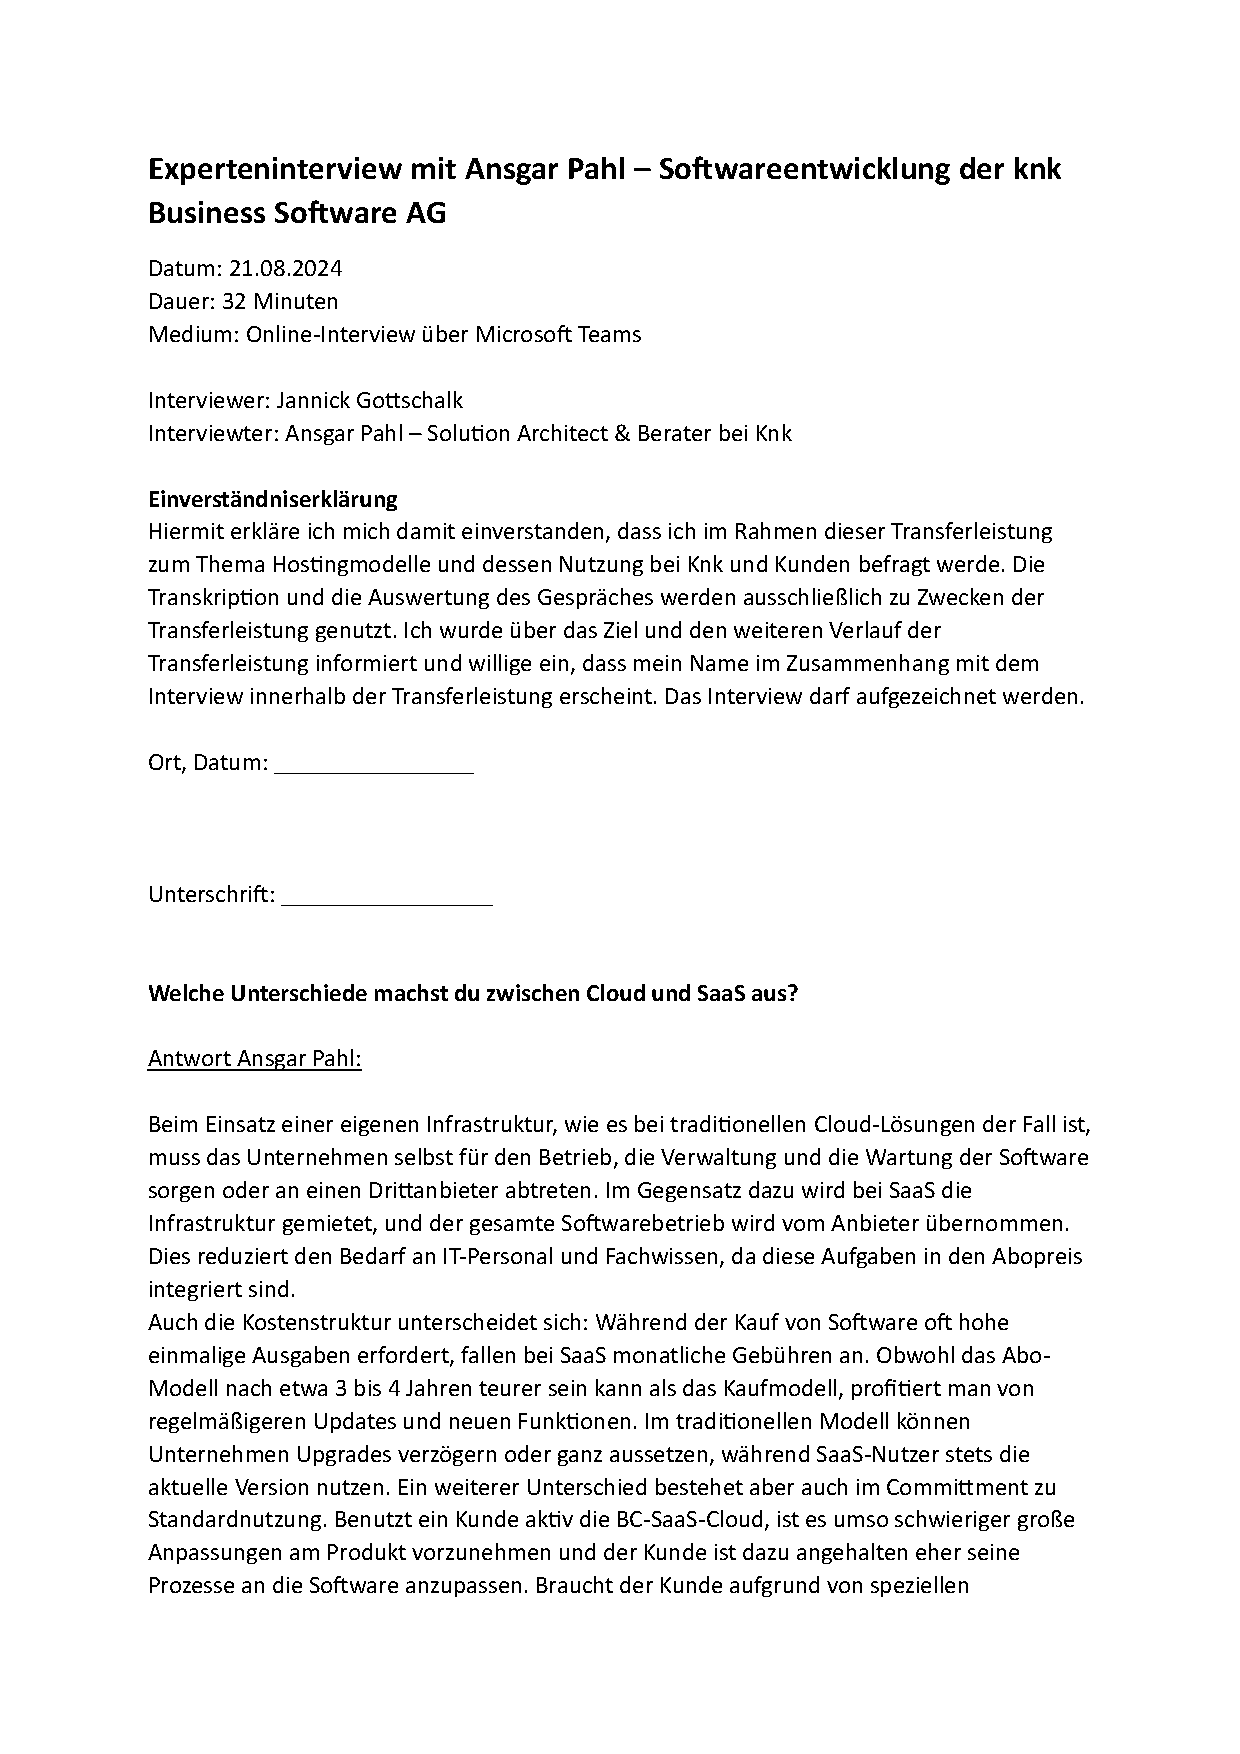
\includepdf[pages=-,picturecommand*={\label{MEINPDFDOKUMENT}}]{Content/Documents/PDF/21.08.2024 Experteninterview mit Ansgar Pahl (nicht unterschrieben).pdf}

\end{document}